% !TeX encoding = UTF-8
% !TeX spellcheck = en_US


%----------------------------------------------------------------------------------------
%	PACKAGES AND OTHER DOCUMENT CONFIGURATIONS
%----------------------------------------------------------------------------------------

\documentclass[11pt, notitlepage]{article} % Default font size and suppress title page

\usepackage[utf8]{inputenc} % Required for inputting international characters
\usepackage[T1]{fontenc} % Output font encoding for international characters
% A note on fonts: As of 2019, NIH allows Arial, Georgia, Helvetica, and Palatino Linotype. Georgia and Arial are commercial fonts so you will need to use XeLaTeX and have them installed on your machine to use them. Palatino & Helvetica are available as free LaTeX packages so select the one you want and comment out the other.
\usepackage{palatino} % Palatino font
\linespread{1.05} % A little extra line spread is better for the Palatino font
%\usepackage{helvet} % Helvetica font
\renewcommand*\familydefault{\sfdefault} % Use the sans serif version of the font

\usepackage{amsfonts, amsmath, amsthm, amssymb} % For math fonts, symbols and environments
\usepackage{graphicx} % Required for including images
% Modify vertical space between figure and caption
\setlength{\abovecaptionskip}{3pt plus 3pt minus 2pt} % Chosen fairly arbitrarily
% The default values are 10pt and 0pt. (The plus and minus allows the space to stretch and shrink if needed. The numbers specify how much.)
\usepackage{booktabs} % Nice rules in tables
\usepackage{wrapfig} % Required for text to wrap around figures and tables
%\usepackage[labelfont=bf]{caption} % Make figure numbering in captions bold
\usepackage[top=1in,bottom=1in,left=1in,right=1in]{geometry} % Page margins
\pagestyle{empty} % Suppress headers and footers
\usepackage{titling}

\usepackage[
backend=biber,
style=numeric,
]{biblatex}
\addbibresource{bib.bib} %Imports bibliography file

\pretitle{

\begin{center}  
\vspace{-1in}
\begin{figure}[h]
    \centering
    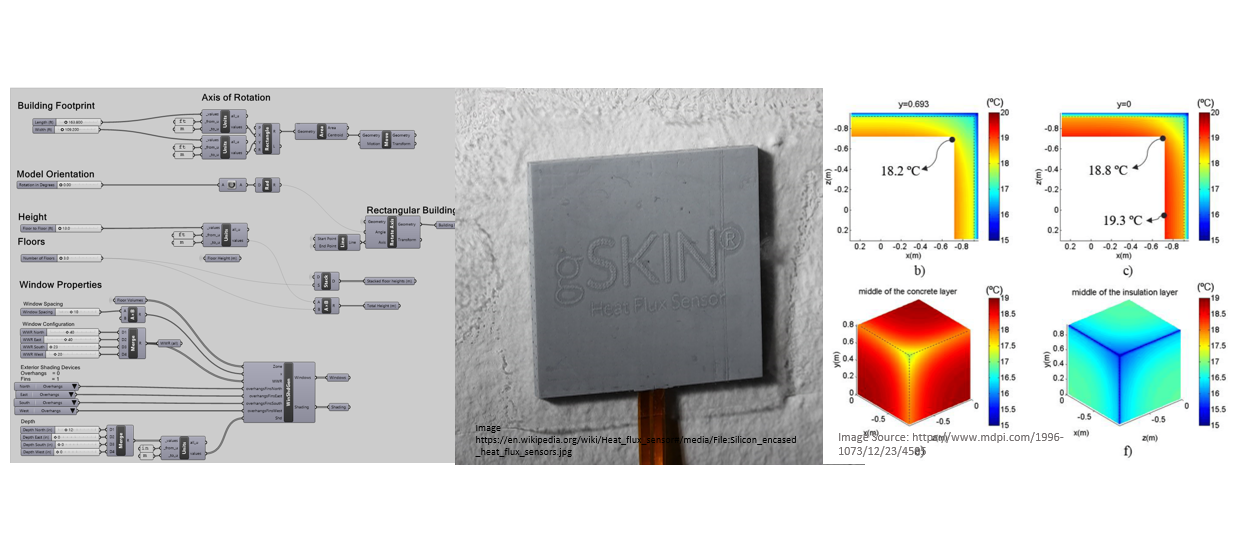
\includegraphics[trim={0 1cm 0 2cm},clip, width=1.0\linewidth]{Headerr.PNG}
    \caption{Grasshopper Visual Programming Script, Heat Flux Sensor, Simulation Output}
    \label{fig:header}
\end{figure}
\vspace{-0.35in}
\end{center}

}

\posttitle{}


%----------------------------------------------------------------------------------------

\begin{document}




\title{
\begin{center}
\noindent\LARGE\textbf{Augmented Architecture: Integrating Numerical Simulations into Regenerative Design}
\end{center}
}
\author{Maryam Almaian, M.S. Architecture}
\date{} % clear date

\maketitle

\vspace{-0.5in}    
Sustainability and awareness about carbon emissions in architecture increase each day, and one of the most critical aspects of carbon emissions is building energy efficiency and thermal comfort. 
However, architect modeling software, such as Rhino, lacks fast 3D heat transfer simulation options. 
Currently, the evaluation of heat transfer is not integrated into the architect's modeling environment and requires avoid cumbersome and time-consuming remodeling of geometries. 
This research project will integrate OpenFOAM, a library for 3D heat transfer analysis, in Rhino \& Grasshopper (a CAD and visual programming environment for architects), where it can promote the planning of regenerative buildings. 

The new software tool will offer several key features, including seamless integration into Rhino \& Grasshopper, thereby allowing for design optimization and early design analysis with real-time performance feedback. 
Based on the literature, the research will positively serve architects and support the development of regenerative buildings in several aspects \cite{kastner2020solving,mantesi2018modelling}. 


To gain further confidence in the simulation output of my software tool, I am asking for funds to carry out extensive validation and testing via a wall-mounted heat flux sensor. 
More particularly, our objective is to validate the transient simulation capabilities of our OpenFOAM simulation engine.
To that end, the heat flux sensors placed indoors and outdoors will provide the heat flux changes throughout the day, which will validate our simulations. 
If funding is secured, it will significantly improve our access to validation data, allowing us to perform rigorous tests of validated cases and ensure full compliance of our tool with industry standards and best practices. 


\subsection*{Primary Goals and Objectives}
\textbf{(1)} Develop the OpenFOAM GUI and integrate into Rhino \& Grasshopper
\textbf{(2)} Purchase and install heat flux sensors in one of the Georgia Tech buildings for a longitudinal experiment.
\textbf{(3)} Improvement transient simulation capability and validate results with on-site measurements
\textbf{(3)} Software tool dissemination in the Food4Rhino\footnote{\url{https://www.food4rhino.com}} Grasshopper software repository. 


\subsection*{Methods}

  %  \item\textbf{Literature Review: } A comprehensive and qualitative review has been conducted to prove the need and role of the 3D heat transfer simulation tool. 
  %  \item\textbf{Case Studies Review and Selection:} Several case studies were reviewed to select the most suitable case for the simulation and testing.

  
\textbf{(1) OpenFOAM Case Setup:} Construct the validated case in OpenFOAM and create the 3D heat transfer solver. 
\textbf{(2) Sensors Installation:} Install the sensors in The Kendeda Building with the cooperation of the building management.
\textbf{(3) Analysis \& Testing:} Analyze, test, and troubleshoot the integrated tool with installed sensors
\textbf{(4) Validation:} Validate the software and experiment, then release publicly via Food4Rhino\footnote{\url{https://www.food4rhino.com}} Grasshopper software repository


\subsection*{Time schedule}
\textbf{Fall 23 --- } Literature review, Case Studies Review, Software Development.
\textbf{Spring 24 --- } Testing and experiments.
\textbf{Summer 24 --- } Validation of simulation results.


\subsection*{Significance of the Research}
\textbf{(1)} Prioritization of energy efficiency in regenerative design will be improved due to thermal comfort and temperature distribution studies in early design. 
\textbf{(2)} Health and well-being of the inhabitants will improve as a result of improved indoor thermal comfort.
\textbf{(3)} A key element of a regenerative building is the ability to withstand extreme climate scenarios---the tool can be used to simulate heat transfer for future climate scenarios, allowing holistic life cycle analyses.
\textbf{(4)} The tool will be made available free of charge to Georgia Tech students and beyond.


\section*{Plans for dissemination of findings}
\textbf{(1)} The main deliverables are a peer-reviewed conference publication in IBPC24\footnote{\url{https://www.ibpc2024.org}};
\textbf{(2)} Packaging of simulation results and validation data for other researchers to reproduce our findings;
\textbf{(3)} Implementation of the software tool in the Rhino \& Grasshopper visual programming environment.


\subsection*{Other info}

Quoted price for the wall heat flux sensor is \$374\footnote{\url{https://www.omega.com/en-us/temperature-measurement/temperature-surface-sensors/p/UHF-HFS-Series}}. Kastner lab (School of Architecture) will fund the remaining \$622 not covered by a grant to acquire three wall heat flux sensors.




\printbibliography




\end{document}